\documentclass{beamer}

\mode<presentation>
{%
	\usetheme{Warsaw}
	\setbeamercovered{invisible}
}
\setbeamertemplate{caption}[numbered] 
\setbeamerfont{caption}{size=\scriptsize}

\usepackage[spanish]{babel}
\usepackage[utf8]{inputenc}
\usepackage{url}
\usepackage{subfig}

\title{Managing the Development of Large Software Systems}

\author[Pipe \& Filter]{%
	{\Large Pipe \& Filter} \\ \vspace{1em}
	Martín Fixman\inst{1} \and
	Ignacio Harari\inst{1} \and \\
	Damián Alemán\inst{1} \and
	Martín Arjovsky\inst{1}
}
\institute{\inst{1} Facultad de Ciencias Exactas y Naturales}

\date{Primer Cuatrimestre 2016}

\begin{document}

\begin{frame}[fragile]
\titlepage{}
\end{frame}

\section{Introducción}

\begin{frame}[fragile]{Introducción}

Esta presentación demuestra algunas observaciones sobre la administración de proyectos como presentado en el paper del {\large Dr.\ Winston W.\ Royce}\cite{royce70}.

\bigskip

En este, se presenta un proceso para mejorar los pasos a seguir durante la administración de un proyecto grande para prevenir errores y lograr bajar los costos de corregirlos cuando ocurren.

\end{frame}

\begin{frame}
Winston W. Royce (1929 – 7 de junio de 1995)

\begin{itemize}

\item Fue un computólogo Americano, director en el Centro de Tecnología de Software Lockheed en Austin, Texas.

\item Fue el primero en describir ``modelo en cascada'' para el desarrollo de software, aunque: 
\begin{itemize}
\item Royce no utilizo el termino ``cascada'' el ar paper
\item Ni lo propueso como metodología de trabajo.
\end{itemize}
\end{itemize}

\end{frame}


\section{Administración en sistemas pequeños}

\begin{frame}[fragile]
%Hay dos pasos esenciales que son comunes entre todos los desarrollos de programas de computadora: un paso de análisis, y uno de código. Si el programa es lo suficientemente pequeño y el producto final va a ser operado por los que lo construyeron, como suele suceder con los programas de uso interno, puede ser que esto sea todo lo que esté requerido.

\begin{figure}[h]
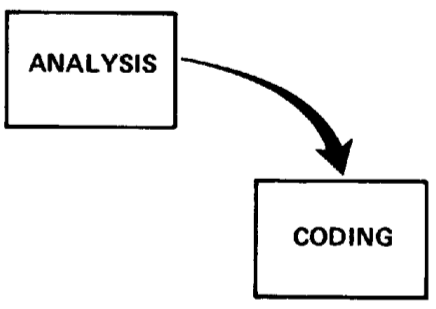
\includegraphics[width=.3\textwidth]{figures/small.png}

\caption{Implementación de un programa pequeño de operaciones internas}
{}
\end{figure}

\vspace{-1em}

Un plan para hacer sistemas más grandes que se base en estos pasos está condenado al fracaso, ya que ante cualquier error o eventualidad es necesario rehacer todo el procesos desde cero.


\end{frame}

\section{Administración en sistemas grandes}

\subsection{Pasos a seguir}
\begin{frame}
Para hacer un proyecto más grande necesitamos:

\begin{itemize}
\item Primero diseñar % Program design comes first
\item Documentar el diseño %Document the design 
\item Hazlo dos veces %Do it twice % 
\item Planear, controlar y monitorear el testeo % Plan, control and monitor testing % Testear
\item Involucrar al cliente %&Involve the customer %
\end{itemize}

\end{frame}

\subsubsection{Primero el diseño}

\begin{frame}{Primero diseñar}

\end{frame}

\subsection{Documentar el diseño}

\begin{frame}{Documentar el diseño}

\end{frame}

\subsubsection{Hazlo dos veces}
\begin{frame}{Hazlo dos veces}

%begin{figure}[h]
%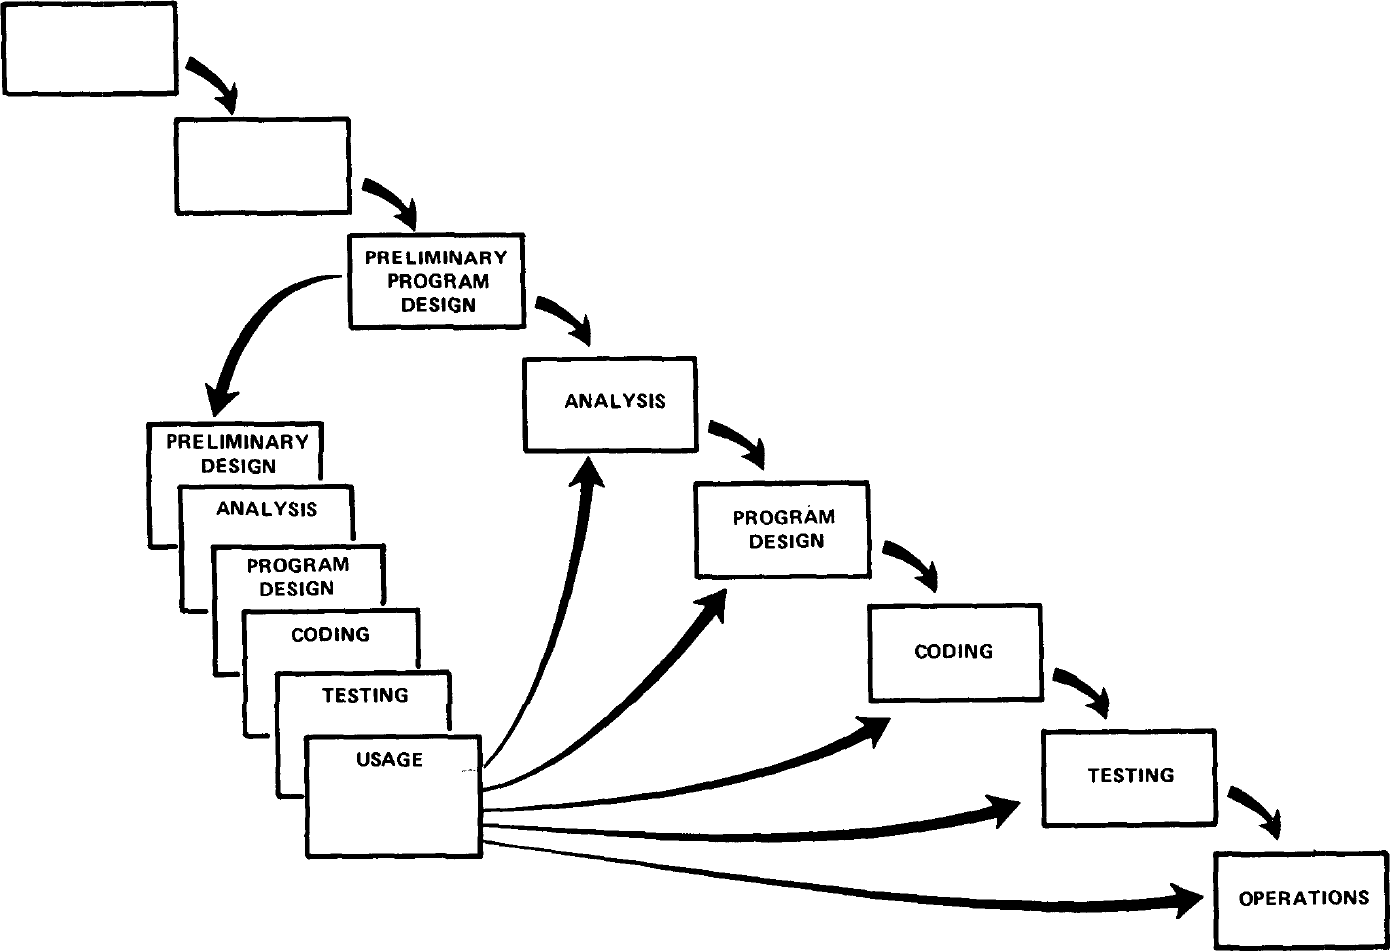
\includegraphics[width=.3\textwidth]{figures/hazloDosVeces.png}
%\end{figure}


\end{frame}

\subsubsection{Testear}

\begin{frame}{Testear}

\end{frame}


\subsubsection{Involucra al cliente}

\begin{frame}{Involucra al cliente}

\end{frame}


\section{Bibliografía}

\begin{frame}[fragile]
\begin{thebibliography}{9}
\bibitem{royce70}
  \footnotesize
  Dr.\ Winston W.\ Royce \\
  \emph{Managing the Development of Large Software Systems} \\
  \texttt{IEEE Wescon},
  August 1970. \\
  \textit{Copyright ®1970 The Institute of Electrical and Electronics Engineers} \\
  {\scriptsize\url{https://cs.umd.edu/class/spring2003/cmsc838p/Process/waterfall.pdf}}
\end{thebibliography}
\end{frame}

\end{document}
